\documentclass{article}

\usepackage[portuguese]{babel}

\usepackage{amsmath, amssymb}
\usepackage{graphicx}
\usepackage{listings}
\usepackage[colorlinks=true, allcolors=blue]{hyperref}

\usepackage[section]{placeins}

\title{Relatório 08}
\author{Vinícius de Oliveira Peixoto Rodrigues (245294)}
\date{Outubro de 2022}

\begin{document}
\maketitle

\section*{Item (a)}

O programa cria um processo-filho, que "recebe a tarefa" de dormir por 6 segundos. O processo-pai, após o \texttt{fork}, dorme por aproximadamente 1 segundo e em seguida termina sua execução sem esperar pela finalização do filho. Enquanto isso, o processo-filho ainda está rodando, e termina sua execução somente após a morte do pai.

\begin{figure}[!ht]
    \begin{center}
        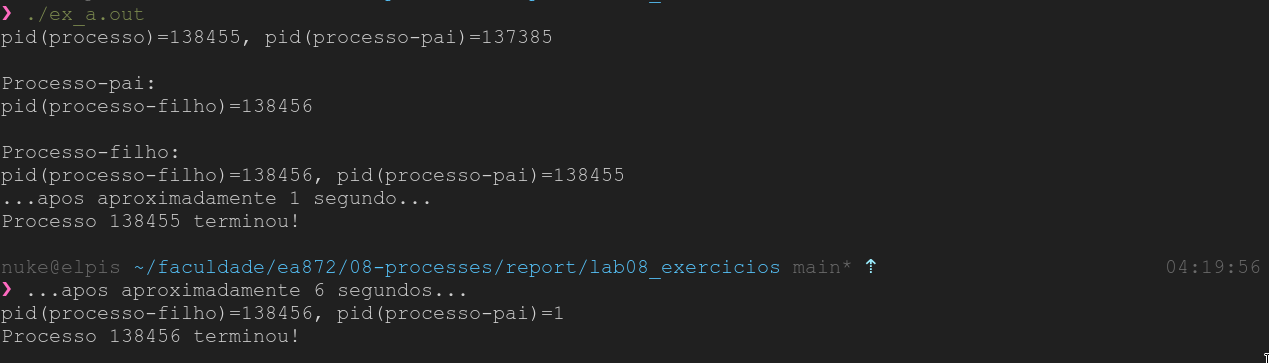
\includegraphics[width=\textwidth]{images/item_a.png}
    \end{center}
\end{figure} 
\FloatBarrier

\section*{Item (b)}

\begin{figure}[!ht]
    \begin{center}
        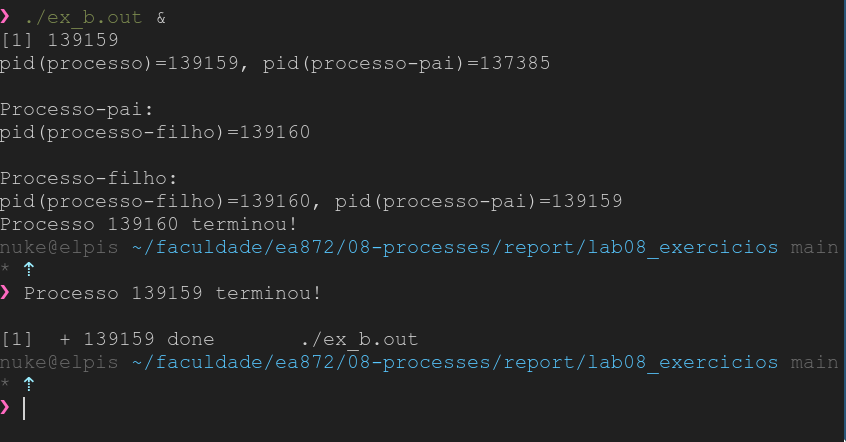
\includegraphics[width=\textwidth]{images/item_b1.png}
    \end{center}
\end{figure} 
\FloatBarrier
\begin{figure}[!ht]
    \begin{center}
        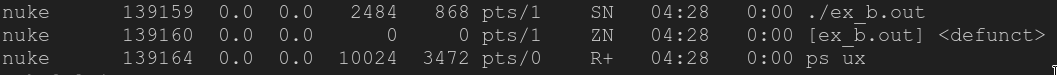
\includegraphics[width=\textwidth]{images/item_b2.png}
    \end{center}
\end{figure} 
\FloatBarrier

O processo-filho se encerra antes do pai e entra no estado \texttt{zombie} (i.e., "dead but not reaped"), visto que o processo-pai não usou a syscall \texttt{wait} para ler o estado de saída do processo-filho. O processo-filho só é limpo após a morte do processo-pai (que implica na terminação/cleanup de todos os childs).

\section*{Item (c)}

A mensagem não aparece porque o primeiro processo-filho termina por meio da chamada \texttt{exit} imediatamente após sair do \texttt{sleep} (e antes de chegar no \texttt{printf} fora do escopo do primeiro condicional).

Além disso, os processos não entram no estado \texttt{zombie} porque foi usada a syscall \texttt{wait} para esperar pela finalização dos dois processos-filhos (de modo que o processo-pai permanece vivo durante toda a duração dos processos-filhos).

\newpage
\section*{Item (d)}

O programa spawna um child process que chama a syscall \texttt{execlp(const char *file, const char *arg, ...)}, que troca a imagem do programa atual pela imagem do programa identificado por \texttt{file}, usando \texttt{arg} como o \texttt{argv[0]} do programa e os argumentos variádicos em \texttt{...} como o restante dos argumentos. 

Enquanto isso, o processo-pai mede o tempo de execução do processo filho (marcando o timestamp de início, depois esperando pelo processo filho com a syscall \texttt{wait}, e depois marcando o timestamp de quando a chamada \texttt{wait} termina).

A diferença do tempo de execução se deve ao fato de que o tempo de CPU usado é definido de forma não determinística pelo \texttt{scheduler} e varia dependendo da quantidade/uso de CPU dos outros processos rodando no sistema.

\begin{figure}[!ht]
    \begin{center}
        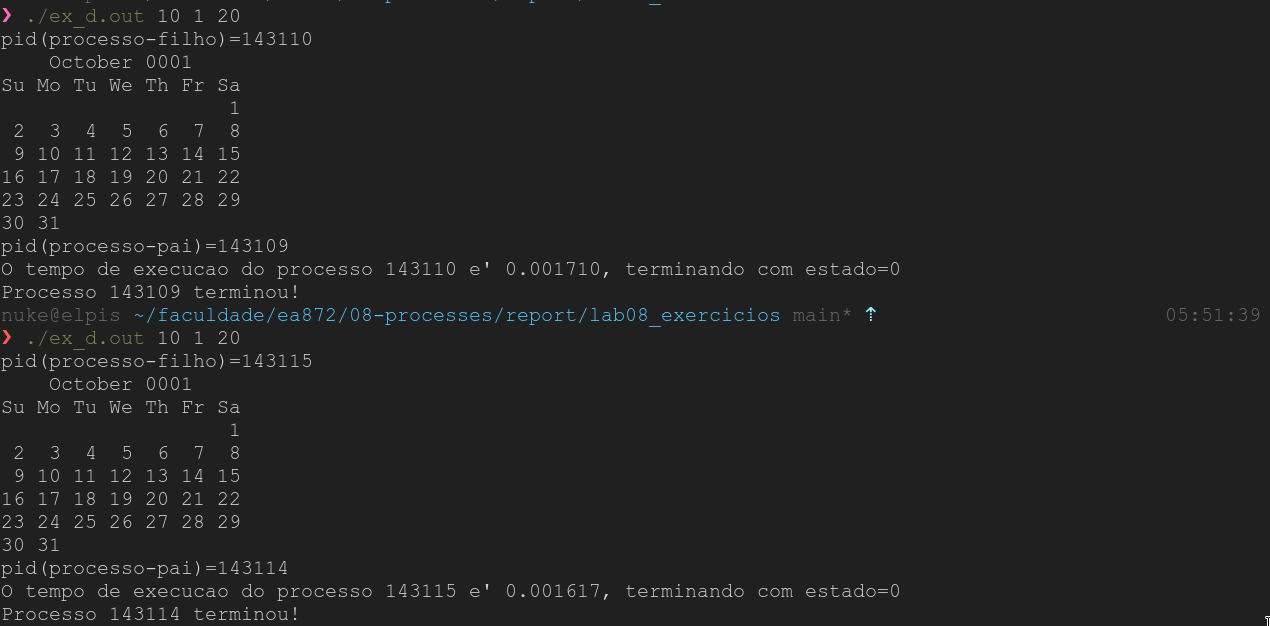
\includegraphics[width=\textwidth]{images/item_d.png}
    \end{center}
\end{figure} 
\FloatBarrier

\newpage
\section*{Item (e)}
\begin{figure}[!ht]
    \begin{center}
        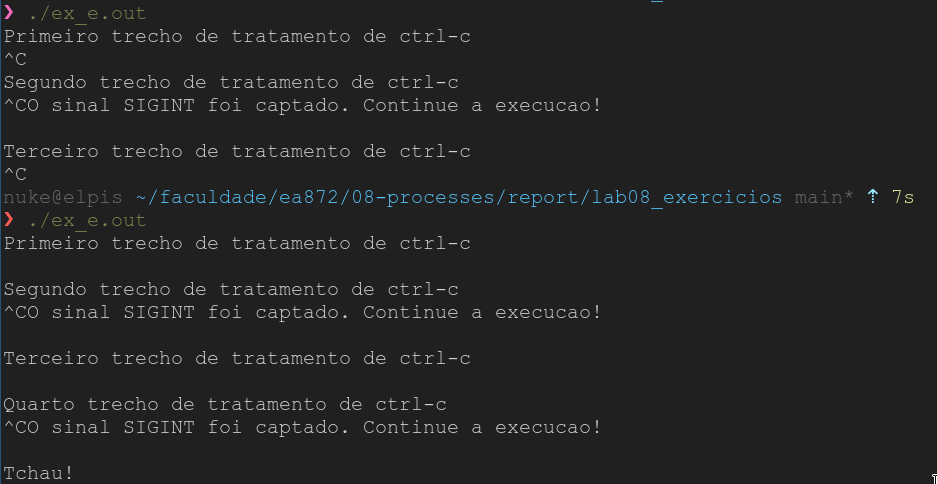
\includegraphics[width=\textwidth]{images/item_e.png}
    \end{center}
\end{figure} 
\FloatBarrier

Primeiramente, é criado um ponteiro de função \texttt{void (*ger\_antiga)()} (isto é, ponteiro para uma função de tipo \texttt{void} que não recebe argumentos). Esse tipo é "compatível" com o tipo \texttt{void (*sighandler\_t)(int)}, que define os handlers de signals registrados por meio da chamada \texttt{signal()}.

Em seguida, são registrados, em intervalos de 5s, três handlers diferentes para o sinal \texttt{SIGINT}:

\begin{enumerate}
    \item \texttt{SIG\_IGN}, que sinaliza que o signal \texttt{SIGINT} deve ser ignorado;
    \item \texttt{ger\_nova}, que printa a mensagem \texttt{"O sinal SIGINT foi capturado..."}
    \item \texttt{SIG\_DFL}, que é o default handler para o signal \texttt{SIGINT} (simplesmente aborta a execução do processo)
    \item o endereço do handler \texttt{ger\_nova} é copiado para o ponteiro \texttt{ger\_antiga}, de modo que a segunda e quarta execução de handlers são iguais (o código que consta no roteiro guarda o default handler \texttt{SIG\_DFL} no ponteiro, mas o código fonte fornecido no Moodle guarda o \texttt{ger\_nova}).
\end{enumerate}

\newpage
\section*{Item (f)}
\begin{figure}[!ht]
    \begin{center}
        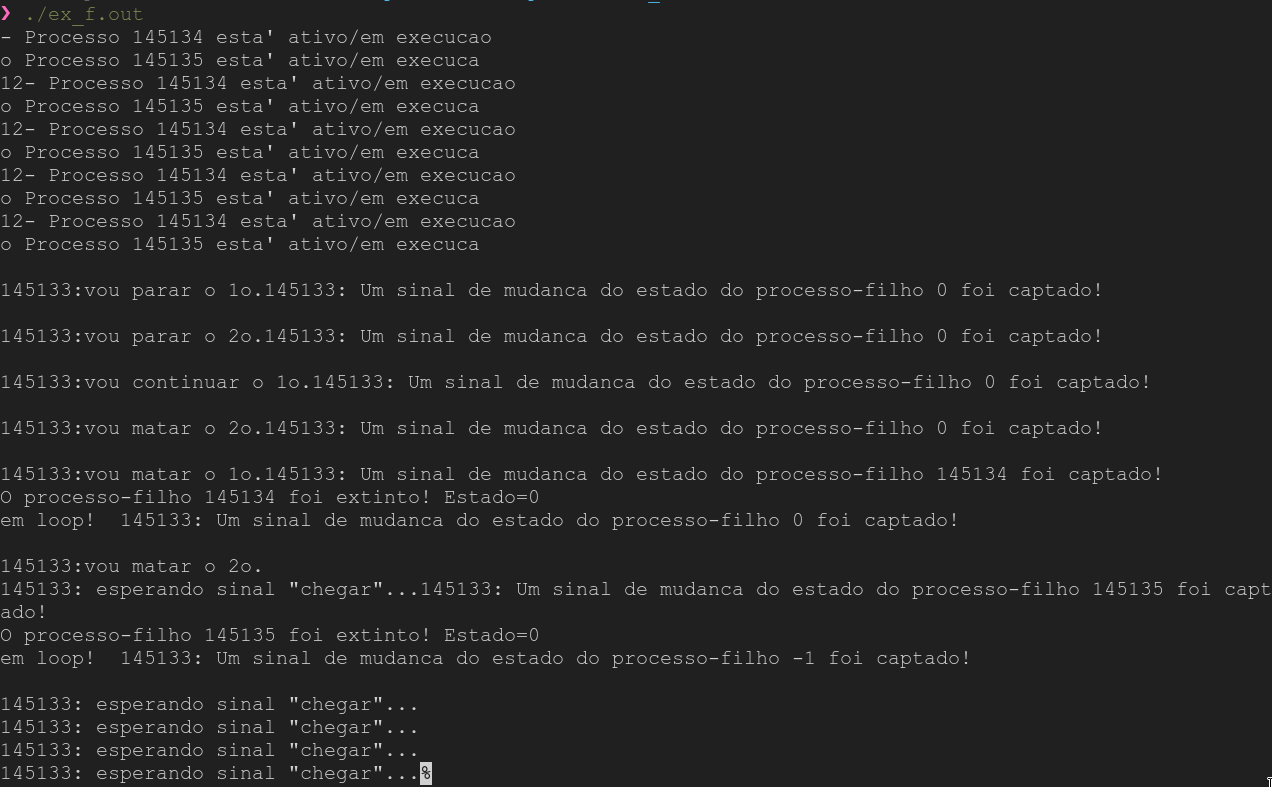
\includegraphics[width=\textwidth]{images/item_f.png}
    \end{center}
\end{figure} 
\FloatBarrier

A chamada \texttt{wait3} é uma interface antiga e deprecada que hoje em dia foi substituída interface mais moderna \texttt{waitpid}; ela serve para capturar uma mudança de estado em qualquer um dos filhos de um processo. As diferenças principais entre ela e a chamada \texttt{wait} são que:

\begin{enumerate}
    \item \texttt{wait3} por padrão espera pela terminação de um processo filho (pode ser alterado por meio do uso de flags)
    \item \texttt{wait3} pode ser non-blocking por meio do uso de flags
\end{enumerate}

Se eliminarmos a linha com a chamada \texttt{wait3}, o valor de \texttt{pid} fica inicializado como lixo de memória (provavelmente com um valor maior que 0), de modo que o programa fica preso em um loop infinito no sighandler.

\end{document}
